\chapter{Background from the main beam dumps}
\label{BeamDumps}

\begin{chapterabstract}
 After every beam collision, the beams of a linear collider are dumped into the main beam dumps.
 For the International Linear Collider, the main beam dump design is based on a water tank, which is tailored to absorb the beam power over a length of about \textit{\SI[detect-all]{12}{\meter}}.
 The first part of this chapter is focused on the irradiation of the water tank and its surrounding, as well as on the neutrons that are produced due to the interaction of the beam particles with the water molecules.
 The second part of this chapter discusses those neutrons which are directed backwards and reach the interaction region.
 They present an additional background for the experiments.
 In the end, suggestions for alternative beam dump designs are given.
\end{chapterabstract}

The spent \positron\electron beams are directed through the extraction line (EXT) of the ILC towards the main beam dumps. 
As can be seen in Figure~\ref{fig:BeamDumps:IP_to_Dump}, the beam dump halls are about \SI{300}{\meter} away from the interaction point (IP) in a direct line of sight.
The extraction lines have the task to transport the highly disrupted beams to the dumps, because of which their quadrupole magnets have a large acceptance for offsets in the beam orbit as well as in the beam momentum of up to \SI{60}{\percent}~\cite[p. 139]{TDR32}.
The quadrupole magnets are to minimize beam loss so that additional diagnostic devices in the EXT lines can measure the qualities of beam bunches before they are dumped.
\begin{figure}
\centering
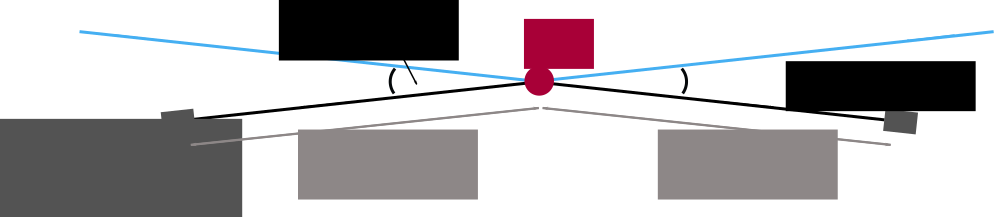
\includegraphics[width=0.6\textwidth]{Figures/BeamDump/IP_EXT.png}
\caption[Schematic of the ILC interaction region with extraction line]{Illustration of the interaction region of the ILC with the extraction line (EXT) leading from the IP to the main beam dump halls.
The extraction lines are about \SI[detect-all]{300}{\meter} long.
The illustration is not to scale.}
\label{fig:BeamDumps:IP_to_Dump}
\end{figure}
\\The beam dump designs are based on water tanks, which are surrounded by iron and concrete shielding walls. 
The two different designs, which are studied in this chapter, are described in detail in Section~\ref{BeamDumps:design}.
The choice of a water tank as the beam dump is motivated by the high specific heat capacity of water, which is ideal to dissipate the energy of the beams. 
The water beam dumps for the ILC have to be able to absorb a beam power of up to about \SI{17}{\mega\watt}\footnote{This value includes the average beam power of \SI{13.7}{\mega\watt} at a center-of-mass energy of \SI{1}{\TeV} plus safety margins of \SI{20}{\percent}.} for the ILC stage at a center-of-mass energy of \SI{1}{\TeV}~\cite{BeamDumpSpecs}.
\\The high energy lepton beam interacts with the water molecules, leading to the emission of neutrons under all solid angles. 
Not only the effect of these neutrons reaching back to the interaction region, but also the doses that the surrounding area would suffer from, are the center of interest in this chapter. 
The rise in the occupancy of the detector experiments is one effect of the neutrons, whereas the damage of the detector components is another severe consequence.
The neutron background would on the one hand lead to displacement damage in the silicon sensors, which results in charge traps, reduction of charge transfer and the overall degrading of the detector performance. 
On the other hand, the immediate irradiation of the beam dump surrounding leads to restricted access for the maintenance staff and personnel.
\\It is therefore crucial to understand the irradiation and the level of neutron background generated by every beam pulse dumped into the ILC main beam dumps.

\section{\fluka and \flair}
\label{BeamDumps:fluka}
The simulation study of the ILC main beam dumps for this thesis was done using the Monte Carlo simulation tool \fluka~\cite{FLUKA,FLUKA2}.
\fluka calculates the particle transport and interactions with matter of the user-defined geometry.
With the graphical interface \flair~\cite{FLAIR}, which was specifically developed for \fluka, complex geometries can be constructed with the help of technical drawings that can be imported as templates into the \flair-geoviewer plug-in (see Figure~\ref{fig:BeamDumps:geoviewer}).
It allows interactive geometry viewing and editing, as well as debugging and three dimensional visualization.
\\\fluka's capabilities cover furthermore the calculation of particle densities and energy densities, the activation of material, and the residual dose rates when considering variable cooling times.
These functionalities were used for the study of the ILC beam dump designs presented in the following sections.
\begin{figure}[hbp]
\centering
\includegraphics[width=0.5\textwidth]{Figures/BeamDump/Design2_geometry_drawing_xz.png}
\caption[Preview of the geometry construction in \flair]{Preview of the construction of the ILC beam dump using a technical drawing as a template imported into the \flair-geoviewer plug-in.}
\label{fig:BeamDumps:geoviewer}
\end{figure}

\section{ILC main beam dump designs}
\label{BeamDumps:designs}
The designs for the main beam dump in this study are based on the technical design drawings done by Benjamin Smith~\cite{Smith_drawings}.
The drawings include plans for the surface building, the beam dump hall with the shielding walls around the water tank, and two different designs for the main beam dumps.
The design based on the drawing with the identification number 0-TB-0067-210-00-A shall henceforth be called ``Design 1'', the second design based on drawing 0-TB-0067-300-00-A shall be called ``Design 2''.
Figure~\ref{fig:BeamDumps:geometry} shows a visualization of the beam dump hall modeled within \fluka. 
It is a simplified version, only containing a simple water tank in the middle of the shielding in the beam dump tomb. 
The infrastructure, such as cables and water pipes, is not included in the simulation geometry.
\\As mentioned in the section above, technical design drawings can be imported into \flair, and directly used as templates for the construction of the geometry.
This was done for the two beam dump designs, which will be explained in detail in the following.
\begin{figure}[hbp]
\begin{center}
\resizebox{.9\textwidth}{!}{%
\includegraphics[height=0.35\textheight]{Figures/BeamDump/Front_view_BeamDump_Tomb.png}%
\quad
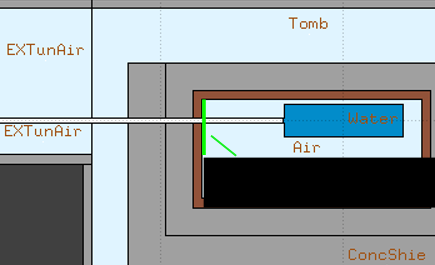
\includegraphics[height=0.35\textheight]{Figures/BeamDump/Bird_view_BeamDump_Tomb.png}%
}
\caption[Geometry visualization of the ILC main beam dump hall]{The beam dump hall was modeled within \fluka and visualized with \flair.
The left hand picture is the front view, the beam direction is going into the page.
The right hand figure shows the top view, in which the water tank is shown in the middle of the different shielding walls. 
A \fluka specific feature is the need of having a black body void around the geometry. 
This void is the boarder of the tracking region, and stops all particles reaching this edge.}
\label{fig:BeamDumps:geometry}
\end{center}
\end{figure}

\subsection{Design 1}
\label{BeamDumps:design:design1}
As both beam dump designs are based on a water tank system, their basic layout is very similar.
For both, the water vessel out of 316L stainless steel has a diameter of \SI{1.5}{\meter} and a length of \SI{6.5}{\meter}.
The water is pressurized to \SI{10}{\bar}.
\\The window between the vessel and the beam pipe has a diameter of \SI{30}{\centi\meter} and a thickness of \SI{1}{\milli\meter}.
For its material, the titanium alloy Ti-6Al-4V is foreseen.
\\Overall, the water volume represents a radiation length of \SI{27}{\xzero}.

\subsection{Design 2}
\label{BeamDumps:design:design2}

\section{Simulation studies of the beam dump surrounding}
\label{BeamDumps:sim_surrounding}

\begin{itemize}
 \item Energy deposition for both designs - done
 \item Dose rate for both designs - done 
 \item Particle fluxes for both designs - done 
 \item Number for certain subregions - almost done
 \item Neutron spatial distributions - almost done
\end{itemize}


\section{Simulation studies of extraction line}
\label{BeamDumps:sim_EXT}

\begin{itemize}
 \item Extraction line lattice - explain components
 \item Simulation of neutrons through EXT - not done yet
\end{itemize}

\section{SiD Occupancy study from beam dump neutrons}
\label{BeamDumps:SiDocc}

\begin{itemize}
 \item Occupancy study of neutrons in SiD - not done yet
\end{itemize}